\documentclass[12pt, a4paper, oneside]{ctexart}
\usepackage{amsmath, amsthm, amssymb, bm, color, graphicx, geometry, mathrsfs,extarrows, braket, booktabs, array, wrapfig, enumitem}
\usepackage[colorlinks,linkcolor=red,anchorcolor=blue,citecolor=blue,urlcolor=blue,menucolor=black]{hyperref}
%%%% 设置中文字体 %%%%
% fc-list -f "%{family}\n" :lang=zh >d:zhfont.txt 命令查看已有字体
\setCJKmainfont{方正书宋.ttf}[BoldFont = 方正黑体_GBK.ttf, ItalicFont = simkai.ttf, BoldItalicFont = 方正粗楷简体.ttf]
%%%% 设置英文字体 %%%%
\setmainfont{Times New Roman}
\setsansfont{Calibri}
\setmonofont{Consolas}

%%%% 设置行间距与页边距 %%%%
\linespread{1.4}
%\geometry{left=2.54cm,right=2.54cm,top=3.18cm,bottom=3.18cm}
\geometry{left=1.84cm,right=1.84cm,top=2.18cm,bottom=2.18cm}

%%%% 图片相对路径 %%%%
\graphicspath{{figures/}} % 当前目录下的figures文件夹, {../figures/}则是父目录的figures文件夹
\setlength{\abovecaptionskip}{-0.2cm}  % 缩紧图片标题与图片之间的距离
\setlength{\belowcaptionskip}{0pt} 

%%%% 缩小item,enumerate,description两行间间距 %%%%
\setenumerate[1]{itemsep=0pt,partopsep=0pt,parsep=\parskip,topsep=5pt}
\setitemize[1]{itemsep=0pt,partopsep=0pt,parsep=\parskip,topsep=5pt}
\setdescription{itemsep=0pt,partopsep=0pt,parsep=\parskip,topsep=5pt}

%%%% 自定义公式 %%%%
\everymath{\displaystyle} % 默认全部行间公式
\DeclareMathOperator*\uplim{\overline{lim}} % 定义上极限 \uplim_{}
\DeclareMathOperator*\lowlim{\underline{lim}} % 定义下极限 \lowlim_{}
\DeclareMathOperator*{\argmax}{arg\,max}  % 定义取最大值的参数 \argmax_{}
\DeclareMathOperator*{\argmin}{arg\,min}  % 定义取最小值的参数 \argmin_{}
\let\leq=\leqslant % 将全部leq变为leqslant
\let\geq=\geqslant % geq同理
\DeclareRobustCommand{\rchi}{{\mathpalette\irchi\relax}}
\newcommand{\irchi}[2]{\raisebox{\depth}{$#1\chi$}} % 使用\rchi将\chi居中

%%%% 自定义环境配置 %%%%
\newcounter{problem}  % 问题序号计数器
\newenvironment{problem}[1][]{\stepcounter{problem}\par\noindent\textbf{题目\arabic{problem}. #1}}{\smallskip\par}
\newenvironment{solution}[1][]{\par\noindent\textbf{#1解答. }}{\smallskip\par}  % 可带一个参数表示题号\begin{solution}{题号}
\newenvironment{note}{\par\noindent\textbf{注记. }}{\smallskip\par}
\newenvironment{remark}{\begin{enumerate}[label=\textbf{注\arabic*.}]}{\end{enumerate}}
\BeforeBeginEnvironment{minted}{\vspace{-0.5cm}}  % 缩小minted环境距上文间距
\AfterEndEnvironment{minted}{\vspace{-0.2cm}}  % 缩小minted环境距下文间距

%%%% 一些宏定义 %%%%
\def\bd{\boldsymbol}        % 加粗(向量) boldsymbol
\def\disp{\displaystyle}    % 使用行间公式 displaystyle(默认)
\def\weekto{\rightharpoonup}% 右半箭头
\def\tsty{\textstyle}       % 使用行内公式 textstyle
\def\sign{\text{sign}}      % sign function
\def\wtd{\widetilde}        % 宽波浪线 widetilde
\def\R{\mathbb{R}}          % Real number
\def\N{\mathbb{N}}          % Natural number
\def\Z{\mathbb{Z}}          % Integer number
\def\Q{\mathbb{Q}}          % Rational number
\def\C{\mathbb{C}}          % Complex number
\def\K{\mathbb{K}}          % Number Field
\def\P{\mathbb{P}}          % Polynomial
\def\d{\mathrm{d}}          % differential operator
\def\e{\mathrm{e}}          % Euler's number
\def\i{\mathrm{i}}          % imaginary number
\def\re{\mathrm{Re}}        % Real part
\def\im{\mathrm{Im}}        % Imaginary part
\def\res{\mathrm{Res}}      % Residue
\def\ker{\mathrm{Ker}}      % Kernel
\def\vspan{\mathrm{vspan}}  % Span  \span与latex内核代码冲突改为\vspan
\def\L{\mathcal{L}}         % Loss function
\def\O{\mathcal{O}}         % big O notation
\def\wdh{\widehat}          % 宽帽子 widehat
\def\ol{\overline}          % 上横线 overline
\def\ul{\underline}         % 下横线 underline
\def\add{\vspace{1ex}}      % 增加行间距
\def\del{\vspace{-1.5ex}}   % 减少行间距

%%%% 定理类环境的定义 %%%%
\newtheorem{theorem}{定理}

%%%% 基本信息 %%%%
\newcommand{\RQ}{\today} % 日期
\newcommand{\km}{微分几何} % 科目
\newcommand{\bj}{强基数学002} % 班级
\newcommand{\xm}{吴天阳} % 姓名
\newcommand{\xh}{2204210460} % 学号

\begin{document}

%\pagestyle{empty}
\pagestyle{plain}
\vspace*{-15ex}
\centerline{\begin{tabular}{*5{c}}
    \parbox[t]{0.25\linewidth}{\begin{center}\textbf{日期}\\ \large \textcolor{blue}{\RQ}\end{center}} 
    & \parbox[t]{0.2\linewidth}{\begin{center}\textbf{科目}\\ \large \textcolor{blue}{\km}\end{center}}
    & \parbox[t]{0.2\linewidth}{\begin{center}\textbf{班级}\\ \large \textcolor{blue}{\bj}\end{center}}
    & \parbox[t]{0.1\linewidth}{\begin{center}\textbf{姓名}\\ \large \textcolor{blue}{\xm}\end{center}}
    & \parbox[t]{0.15\linewidth}{\begin{center}\textbf{学号}\\ \large \textcolor{blue}{\xh}\end{center}} \\ \hline
\end{tabular}}
\begin{center}
    \zihao{3}\textbf{第一次作业}
\end{center}\vspace{-0.2cm}
\begin{problem}
证明下面恒等式:
\begin{enumerate}
    \item $(\bd{a}\times \bd{b})\cdot (\bd{c}\times \bd{d}) = (\bd{a}\cdot \bd{c})(\bd{b}\cdot \bd{d}) - (\bd{b}\cdot \bd{c})(\bd{a}\cdot \bd{d})$
    \item $\bd{a}\times(\bd{b}\times \bd{c})+\bd{b}\times(\bd{c}\times \bd{a}) + \bd{c}\times(\bd{a}\times\bd{b})=0$
    \item $(\bd{a}\times \bd{b})\times(\bd{b}\times \bd{c})\times (\bd{c}\times \bd{a}) = (\bd{a}\cdot \bd{b}\times \bd{c})^2$
\end{enumerate}
\end{problem}
\begin{proof}
    1. \vspace{-1.2cm}
    \begin{align*}
        (\bd{a}\times \bd{b})\cdot(\bd{c}\times \bd{d}) =&\ a\cdot(\bd{b}\times (\bd{c}\times \bd{d}))\\
        \xlongequal{\text{二重向量积}}&\ \bd{a}\cdot((\bd{b}\cdot \bd{d})\bd{c} - (\bd{b}\cdot \bd{c})\bd{d})\\
        =&\ (\bd{a}\cdot \bd{c})(\bd{b}\cdot\bd{d}) - (\bd{a}\cdot\bd{d})(\bd{b}\cdot\bd{c})
    \end{align*}

    2. \vspace{-1.2cm}
    \begin{align*}
        &\ \bd{a}\times(\bd{b}\times \bd{c})+\bd{b}\times(\bd{c}\times \bd{a})+\bd{c}\times(\bd{a}\times \bd{b})\\
        \xlongequal{\text{二重向量积}}&\ (\bd{a}\cdot\bd{c})\bd{b}-(\bd{a}\cdot\bd{b})\bd{c}+(\bd{b}\cdot\bd{a})\bd{c} - (\bd{b}\cdot\bd{c})\bd{a}+(\bd{c}\cdot\bd{b})\bd{a}-(\bd{c}\cdot\bd{a})\bd{b}\\
        \xlongequal{\text{内积交换律}}&\ 0
    \end{align*}

    3. \vspace{-1.2cm}
    \begin{align*}
        &\ (\bd{a}\times \bd{b})\cdot(\bd{b}\times \bd{c})\times(\bd{c}\times \bd{a})\\
        =&\ (\bd{a}\times \bd{b})\left[((\bd{b}\times\bd{c})\cdot\bd{a})\bd{c}-((\bd{b}\times\bd{c})\cdot\bd{c})\cdot \bd{a}\right]\\
        \xlongequal{\bd{a}\times\bd{b}\cdot \bd{a} = 0}&\ [(\bd{b}\times\bd{c})\cdot\bd{a}][(\bd{a}\times\bd{b})\cdot \bd{c}]\\
        =&\ (\bd{b}\times \bd{c}\cdot \bd{a})^2 = (\bd{a}\cdot \bd{b}\times \bd{c})^2
    \end{align*}
\end{proof}
\begin{problem}
采用向量方法证明:
\begin{enumerate}
    \item 平面上三角形的三条中线交于一点,这点分中线为1:2两部分,称为三角形的重心.
    \item 空间中四面体的顶点到对面三角形的重心的连线称为四面体的中线. 
    证明四条中线相交于同一个点,称为四面体的重心,并且重心分中线为1:3两个部分.
\end{enumerate}
\end{problem}

\begin{solution}\vspace{-0.5cm}\\
\begin{wrapfigure}[8]{r}{.55\linewidth} % 文字环绕行数为13行, 图片靠右 (l为靠左), 图片占0.5的行宽
    \vspace{-1cm}
    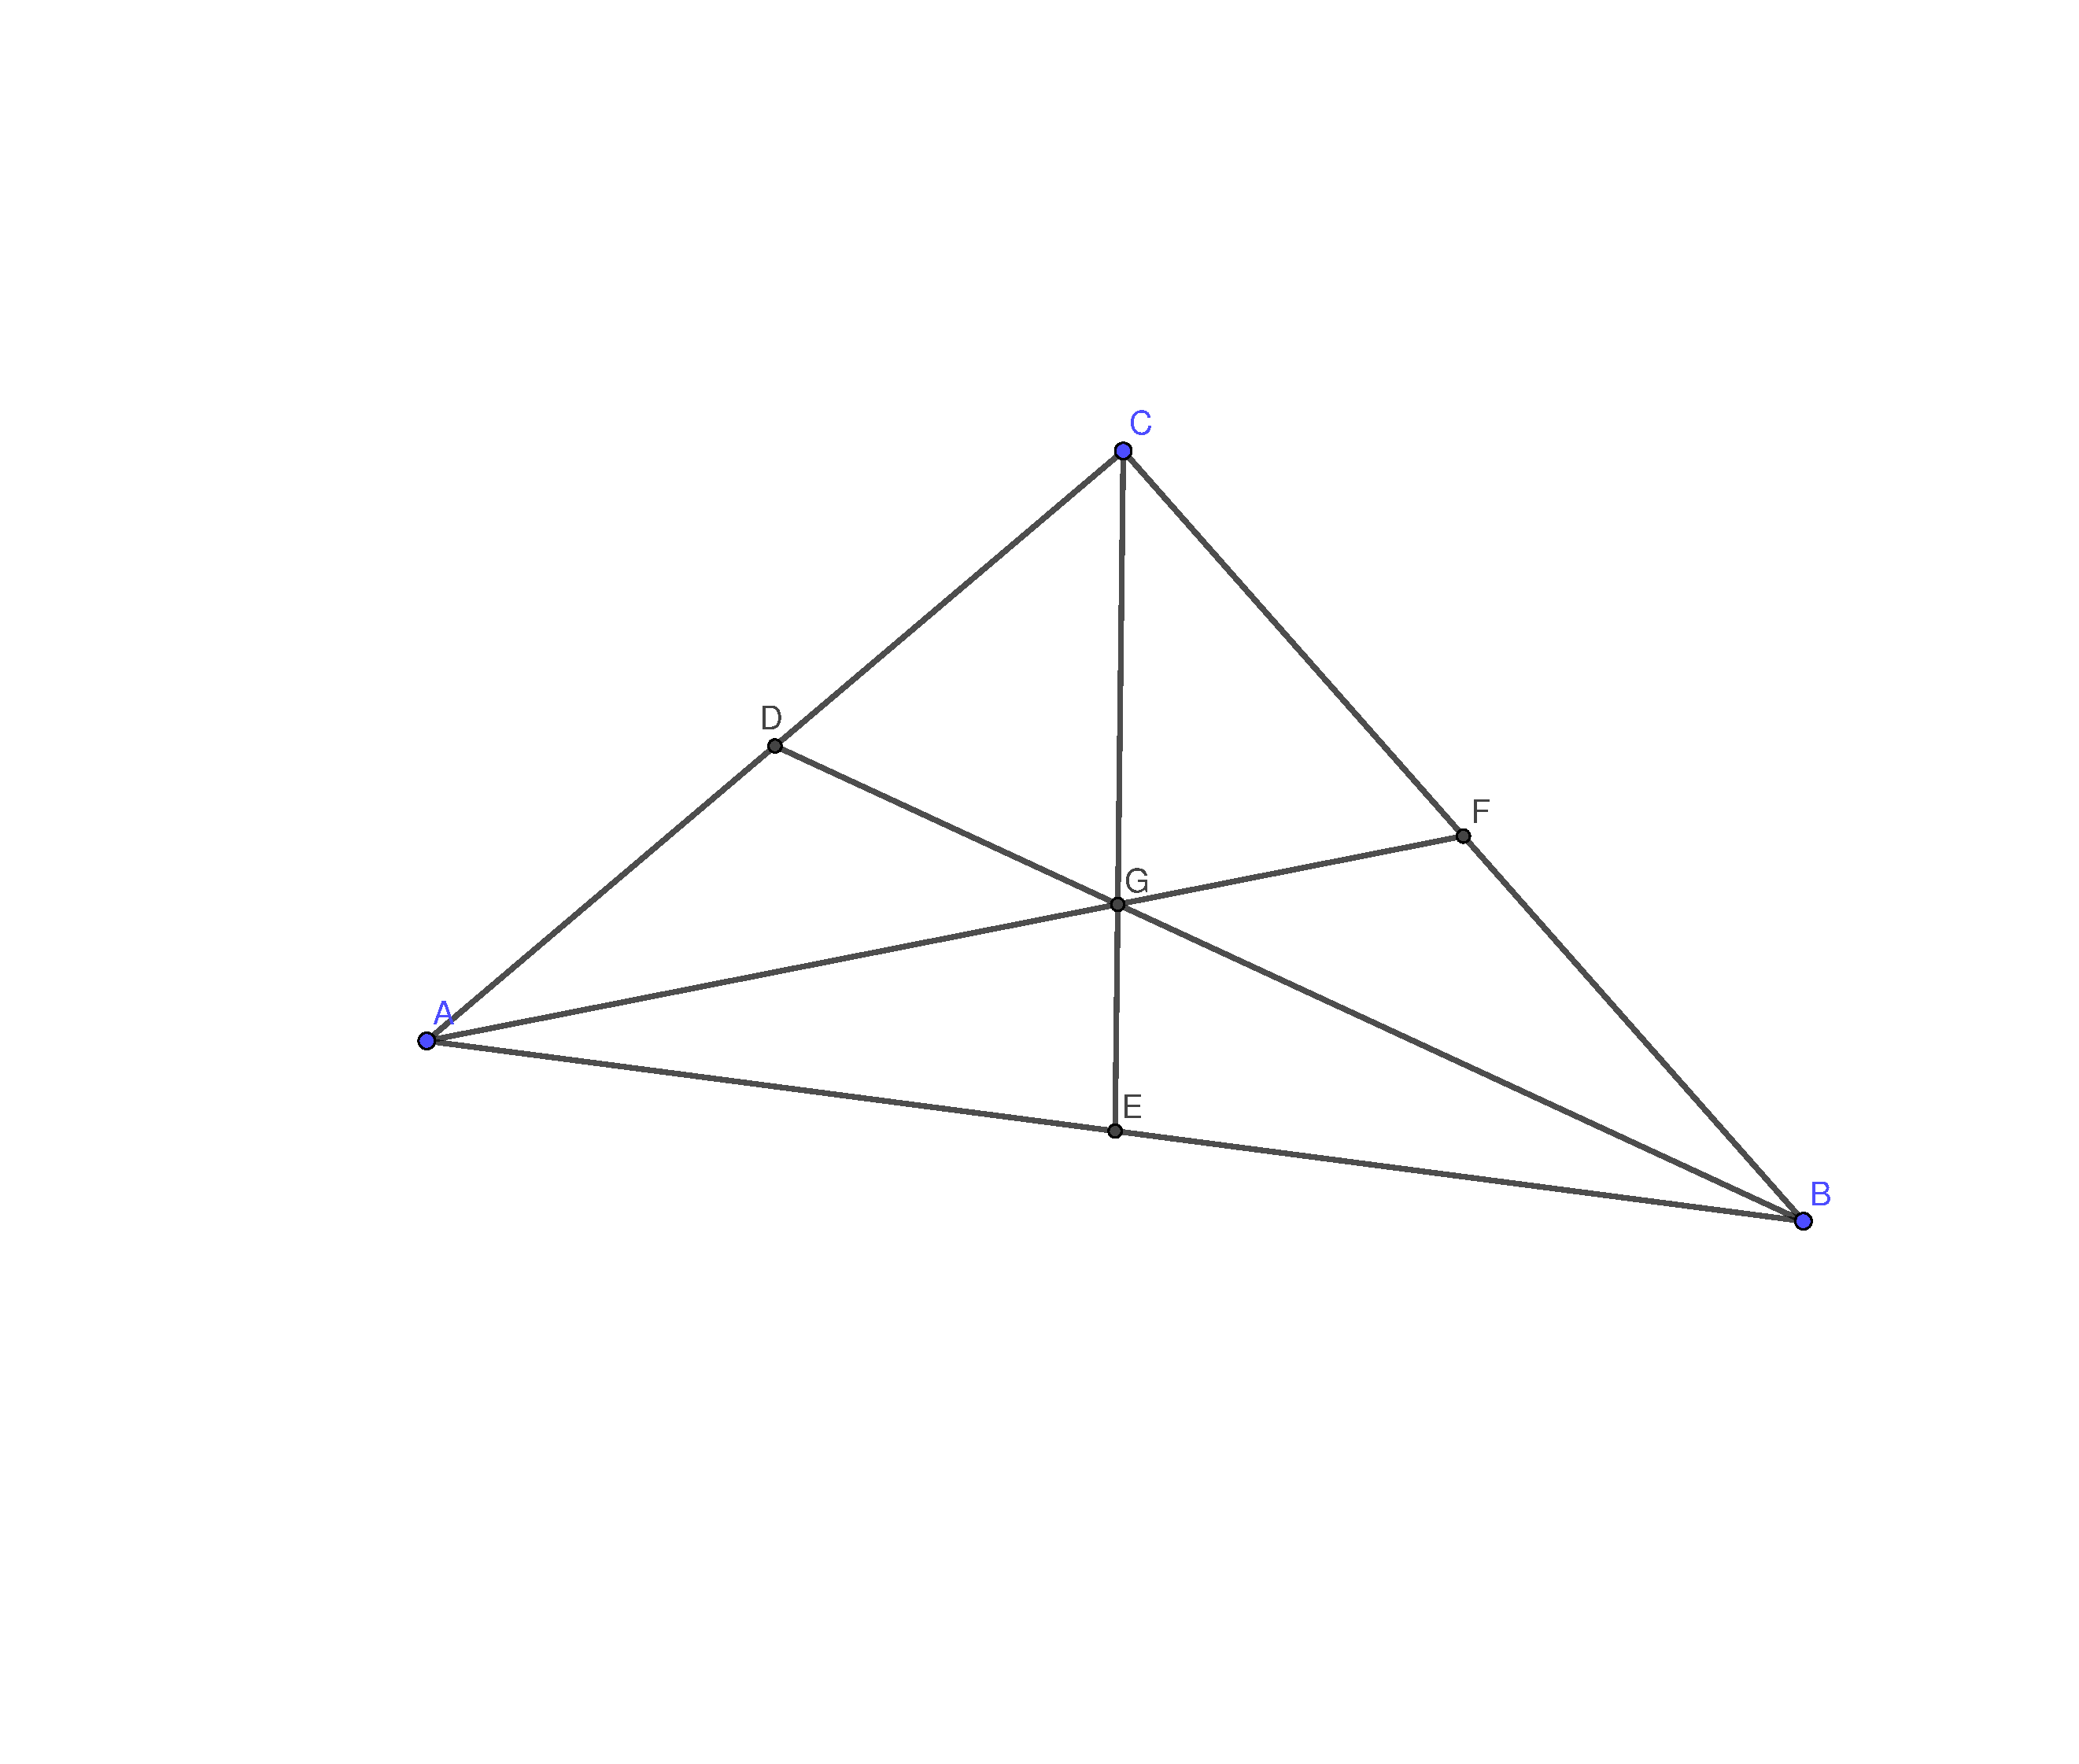
\includegraphics[scale=0.33]{微分几何第一次作业.pdf} % scale=0.7按比例缩放70%
\end{wrapfigure}
1. 以右图三角形$\triangle ABC$为例,$D,E,F$为三边的中点,则$G$为三条重心,设$\overrightarrow{AB} = \bd{a}$,$\overrightarrow{AC} = \bd{b}$,则$\overrightarrow{BC} = \bd{b}-\bd{a}$. 
下证$G$为$AF$的三等分点,由于$\overrightarrow{AF} = \frac{\bd{a}+\bd{b}}{2}$,$\overrightarrow{CE} = \frac{\bd{a}-2\bd{b}}{2}$,设$|AG|:|AF| = \alpha, |CG|:|CE| = \beta$,于是
\begin{equation*}
    \alpha \overrightarrow{AF} + \beta\overrightarrow{EC} = \overrightarrow{AC}
\end{equation*}
也就是
\begin{equation*}
    \alpha\frac{\bd{a}+\bd{b}}{2}+\beta{2\bd{b}-\bd{a}}{2} = \bd{b}\Rightarrow \begin{cases}
        \alpha-\beta = 0,\\
        \alpha+2\beta = 2
    \end{cases}\Rightarrow \alpha = \beta = \frac{2}{3}
\end{equation*}
于是$G$时$AF$的三等分点,类似地,可以证明$G$是$BD$,$CE$的三等分点.

\begin{wrapfigure}[8]{r}{.55\linewidth} % 文字环绕行数为13行, 图片靠右 (l为靠左), 图片占0.5的行宽
    \centering
    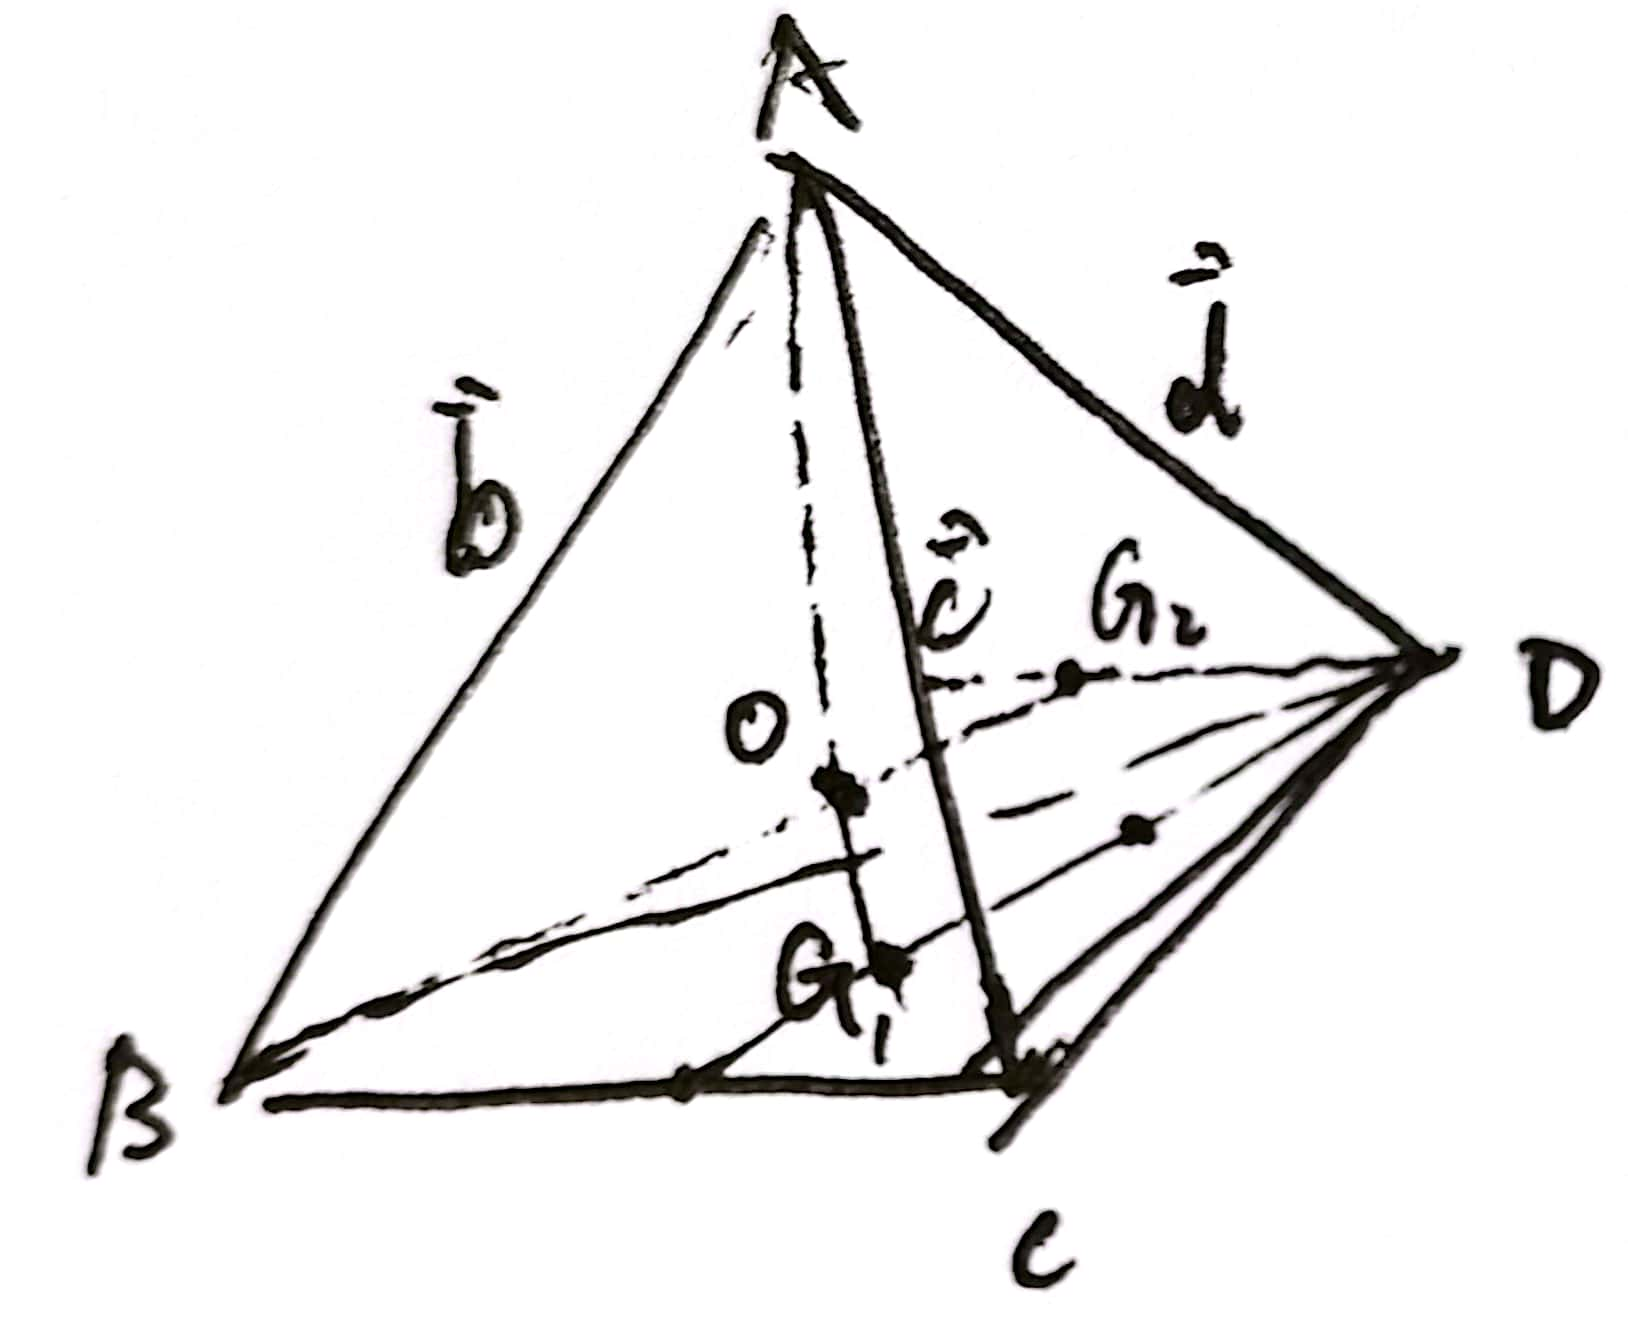
\includegraphics[scale=0.13]{微分几何第一次作业2.jpg} % scale=0.7按比例缩放70%
\end{wrapfigure}
2. 以右图四面体$ABCD$为例,$G_1$为$\triangle BCD$的重心,$G_2$为$\triangle ACD$的重心,设
\begin{align*}
    \overrightarrow{AB} = \bd{b},\ \overrightarrow{AC} = \bd{c},\ \overrightarrow{AD} = \bd{d}
\end{align*}
则$\overrightarrow{BD} = \bd{d} - \bd{b},\ \overrightarrow{CD} = \bd{d} - \bd{c}$,于是
\begin{align*}
    \overrightarrow{DG_1} =&\ \frac{1}{3}(\overrightarrow{DB}+\overrightarrow{DC}) = \frac{1}{3}(\bd{b}+\bd{c}-2\bd{d})\\
    \overrightarrow{DG_2} =&\ \frac{1}{3}(\overrightarrow{DA}+\overrightarrow{DC}) = \frac{1}{3}(\bd{c}-\bd{d})
\end{align*}
则
\begin{equation*}
    \overrightarrow{AG_1} = \overrightarrow{AD} + \overrightarrow{DG_1} = \frac{1}{3}(\bd{b}+\bd{c}+\bd{d}),\quad
    \overrightarrow{BG_2} = \overrightarrow{BD}+\overrightarrow{DG_2} = -\bd{b}+\frac{1}{3}(\bd{c}+\bd{d})
\end{equation*}
假设存在$\alpha,\beta\in\R$,使得$\overrightarrow{AB} = \alpha\overrightarrow{AG_1} + \beta\overrightarrow{G_2B}$,于是
\begin{equation*}
    \frac{\alpha}{3}(\bd{b}+\bd{c}+\bd{d})  + \beta\bd{b} - \frac{\beta}{3}(\bd{c}+\bd{d}) = \bd{b}
    \Rightarrow \begin{cases}
        \alpha/3 + \beta = 1\\
        \alpha/3 = \beta/3
    \end{cases}\Rightarrow\alpha = \beta = \frac{3}{4}
\end{equation*}
故四面体重心是其中线的四等分点.


\end{solution}
\end{document}